\textbf{TODO}

	\section{Simulation model}
\label{sec:simulation_results}
To evaluate the USARSim simulation model,  
a set of maneuvers is flown with the actual AR.Drone and
simulated AR.Drone. The differences between the maneuvers are studied in detail. To enable multiple repetitions of the same maneuver it is
described as a set of time points (milliseconds since initialization) each coupled to a movement command.
We wrote wrappers for the AR.Drone programming interface and for USARSim interface which read these scripts and output a control
signal, using the system clock to manage the timing independently from the game engine and the AR.Drone hardware.
Orientation, altitude and horizontal speed are recorded at a frequency of 200Hz during the maneuvers. These are gathered through the AR.Drone's internal sensors and the build-in algorithms, which are
also used by the controller to operate the drone. The filtered output of the MEMS gyroscope is used
for estimating orientation. The filtered output of the ultrasound distance sensor is used for estimating
altitude. The optical 
flow algorithm using the bottom camera is used for estimating the horizontal (linear
and lateral) speeds. The simulator has equivalent sensors. In addition, simulation can provide ground-truth data. 
Also for the real maneuvers an attempt was made to generate ground truth via an external reference system; the movements were recorded with a synchronized video system consisting of four firewire cameras, capturing images at 20 frames per second at a resolution of $1024 \times 768$ pixels. The position of the AR.Drone 
in each frame has been annotated by hand. 
%However, since the processing of the captured data is not yet complete, results from these trials are not presented in this paper.
%reference?!

Corresponding to NIST guidelines \cite{Jacoff2010STM}
a set of experiments of increasing complexity was performed. For the AR.Drone
four different experiments were designed.
The first experiment is a simple hover, in which the drone tries to maintain its position (both horizontal and vertical). The second experiment is linear movement, where the drone actuates a single movement command. The third experiment is a small horizontal square. The last experiment is a small vertical square.

\subsubsection{Hovering}

Quadrotors have hovering abilities just like a helicopter. The stability in maintaining a hover depends
on environmental factors (wind, underground, aerodynamic interactions) and control software.
%In \cite{Michael2010ra} a
%horizontal positioning error of no more than $2\small{cm}$ and a vertical error of less than $0.6\small{cm}$ are reported for
%a tightly optimized stiff controller. In practice, softer controllers are used which are more robust and can
%recover from larger disturbances. In \cite{How2008} a horizontal and vertical positioning error of no more than $10\small{cm}$ are %reported. 
If no noise model is explicitly added, the USARSim model performs a perfect hover; when no control signal is given the
horizontal speeds are zero and the altitude stays exactly the same.

For the AR.Drone, this is a good zero-order model. One of the commercial features of the AR.Drone is its ease of operation. As part of this feature it
maintains a stable hover when given no other commands, which is accomplished by a visual feedback loop.
%The hover is quite robust and in impromptu
%ad-hoc tests was able to recover from major attitude disturbances up to $\sim45^o$. However, in this section we
%are concerned with the hovering behavior with minor disturbances. 
So, the hovering experiment is performed  
indoors
with an underground chosen to have enough texture for the optical flow motion estimation algorithm.

As experiment the AR.Drone maintains a hover for 35 seconds. This experiment was repeated 10 times,
collecting 60.000 movement samples for a total of 350 seconds. Over all samples the mean absolute error in horizontal
velocity (the Euclidean norm of the velocity vector) is $0.0422\small{m/s}$ with a sample variance of $0.0012\small{m^2/s^2}$. From
the samples we obtain the distribution of the linear and lateral velocity components. 

From the velocity logs the position of the AR.Drone during the 35-second 
flight was calculated. 
%Figure \ref{fig:scatterplot} shows a scatterplot of positions over all flights.
The mean absolute error of the horizontal position is $0.0707\small{m}$ with a sample variance of $0.0012\small{m^2}$.

\begin{comment} % to save some space
\begin{figure}[htb]
\centering
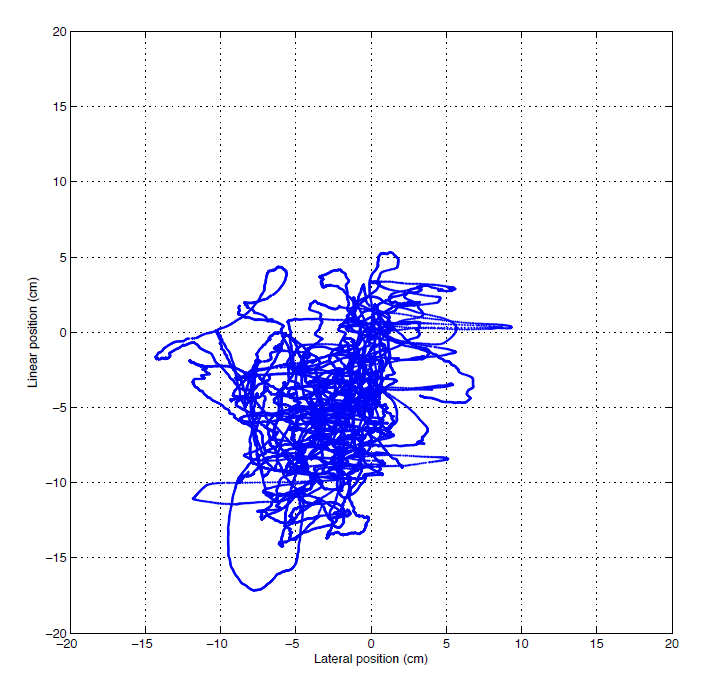
\includegraphics[width=8cm]{images/HoverScatterPlot.png}
\caption{Scatter plot of the horizontal position aggregated over all hover flights.}
\label{fig:scatterplot}
\end{figure}
\end{comment}

\subsubsection{Horizontal movement}

In this experiment the AR.Drone is flown in a straight line. It is given a control pulse (i.e., pitch) with a constant signal
for 5 different time periods: 0.1s, 1s, 2s, 3s, and 5s. Each pulse is followed by a null signal for enough time for the AR.Drone to make a full stop and a negative pulse of the same magnitude for the same period,
resulting in a back and forth movement. In Figure \ref{fig:RealResponse}
 the red line shows the control signal, the blue line the response (i.e., velocity) of the AR.Drone. The experiment was repeated for 5 different speeds.
The control signal $s$ specifies the pitch of the AR.Drone as a factor (between 0 and 1) of the maximum absolute tilt $\theta_{max}$, which was set to the default value\footnote{ARDrone firmware (1.3.3)}. % iPhone uses 12deg
The trials were performed with the
values of 0.05, 0.10, 0.15, 0.20, 0.25 for the control signal $s$.

\begin{figure}[htb]
\centering
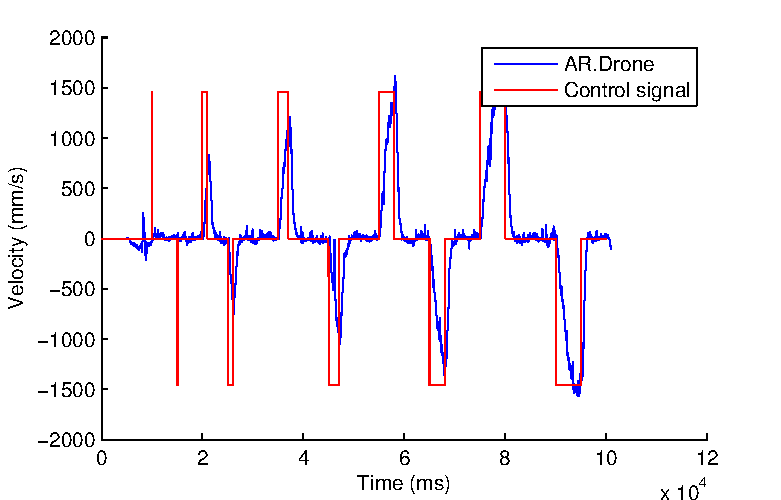
\includegraphics[width=11cm]{images/Dr7Ov-eps-converted-to.pdf}
\caption{Velocity of the real AR.Drone (blue) on a number of control pulses (red) with a pitch of $s=0.15 \times \theta_{max}$ .}
\label{fig:RealResponse}
\end{figure}

Robots in USARSim are controlled with a standardized interface, which uses SI units. A robot in USARSim expects a DRIVE command with a speed in $m/s$ and not the AR.Drone native signal $s$. 
Thus in order to 
fly comparable trials 
the relation between the AR.Drone's angle of attack $\alpha$ and the corresponding velocity $v$ has to be investigated.
When flying straight forward in no-wind conditions, the angle of attack $\alpha$ is equivalent with the pitch $\theta$.
In order to do this the samples from the logs where the AR.Drone has achieved maximum
velocity have to be selected. Closer inspection of the velocity logs show that in each trial there is still constant increase of velocity for the first three pulses. For the last two pulses there is obvious plateauing, which indicates that the last two seconds of the five-second pulses is a good indication for the maximum velocity. Therefore the velocity at those
last two seconds was used to compute mean absolute speeds $\bar{v}$, which are combined with the mean absolute
pitch $\bar{\theta}$ as measured by the MEMS gyroscope. The estimates for $\bar{v}$ and pitch $\bar{\theta}$ are presented in Table~\ref{tab:angle_of_attack} together with their standard deviation. 
% Looking at the values for the pitch we see that these differ from the expected angles listed above.
Extrapolating the mean pitch $\bar{\theta}\simeq7.5^o$ at 
control value $s=0.25$ to the maximum control signal gives an indication of
the AR.Drone's maximum pitch $\theta_{max}\simeq30^o$ value. For typical usage, the angle of attack never exceeds $12^o$ degrees.

\begin{table}[htb]    \centering
    \begin{tabular}
        { | l | l  l  l  l  l | }
        \hline 
          &  \multicolumn{5}{| l |}{Control signal $s$} \\
          & 0.05 & 0.10 & 0.15 & 0.20 & 0.25 \\    
        \hline
        $\bar{v}$ (m/s) & 0.4044 & 0.6284 & 1.4427 & 1.7587 & 2.2094 \\
        $\sigma_v$ (m/s) & 0.096 & 0.226 & 0.070 & 0.126 & 0.165 \\
        \hline
        $\bar{\theta}$ (deg) & 1.4654 & 2.9025 & 4.1227 & 5.7457 & 7.4496 \\
        $\sigma_\theta$ (deg) & 0.455 & 0.593 & 0.482 & 0.552 & 0.921 \\
        \hline
    \end{tabular}    \caption{Averaged velocity $\bar{v}$ measured at the end of a 5 seconds pulse of the control signal $s$, including the corresponding pitch $\bar{\theta}$ as measured by the gyroscope.}
    \label{tab:angle_of_attack}
\end{table}

\begin{comment}
\begin{table}[htb]    \centering
    \begin{tabular} 
        { | l | l | l | l | l | l | }
        \hline 
          &  \multicolumn{5}{|l|}{Control signal $s$} \\
          & 0.05 & 0.10 & 0.15 & 0.20 & 0.25 \\
        \hline
        $\bar{v}$ (m/s) & 0.4044 & 0.6284 & 1.4427 & 1.7587 & 2.2094 \\
        $\sigma_v$ (m/s) & 0.096 & 0.226 & 0.070 & 0.126 & 0.165 \\
        \hline
        $\bar{\theta}$ (deg) & 1.4654 & 2.9025 & 4.1227 & 5.7457 & 7.4496 \\
        $\sigma_\theta$ (deg) & 0.455 & 0.593 & 0.482 & 0.552 & 0.921 \\
        \hline
    \end{tabular}    \caption{Averaged velocity $\bar{v}$ measured at the end of a 5 seconds pulse of the control signal $s$, including the corresponding pitch 
$\bar{\theta}$ as measured by the IMU.} 
    \label{tab:angle_of_attack}
\end{table}
\end{comment}

To convert the AR.Drone's control signal $s$ to USARSim commands $v$ a least-squares fit through the points of Table~\ref{tab:angle_of_attack} is made for the linear function
$v = c \cdot \theta$, which gives us $c=0.2967$. 
Equation \ref{eq:conversion} gives the final conversion of a control signal $s$ to a velocity $v$ in $m/s$ given the
AR.Drone's maximum pitch $\theta_{max}$ in degrees.

\begin{equation}
v = 0.2967 \cdot s \cdot \theta_{max}
\label{eq:conversion}
\end{equation}

The USARSim model has a parameter $P_\theta$ for calculating the angle (radian) given the velocity, which
% we can calculate from the coefficient $c$ above by converting from degrees to radians. This gives us the
% theoretical $P_\theta = \frac{1}{0.2967} \cdot \frac{\pi}{180} = 0.0588$. However, doing a least-squares fit on the angle given the velocity gives 
is the value $\hat{P}_\theta = 0.057$, as used in subsequent simulations.

The next experiment checks the acceleration of the real and simulated AR.Drone. First we give an estimate of how quickly the AR.Drone's controller changes its pitch to match the commanded pitch and how well it can keep it. For this we select all samples from 100ms after the start
of the 2s, 3s and 5s pulses till the first sample at which the commanded pitch has been reached. This
corresponds to the time-span between which the AR.Drone has started to act on the change in the control
signal until it reaches the commanded pitch. The result is illustrated in Figure \ref{fig:ComparisonOfResponse}.
%For each of these spans we estimate the tangent:

\begin{figure}[htb]
\centering
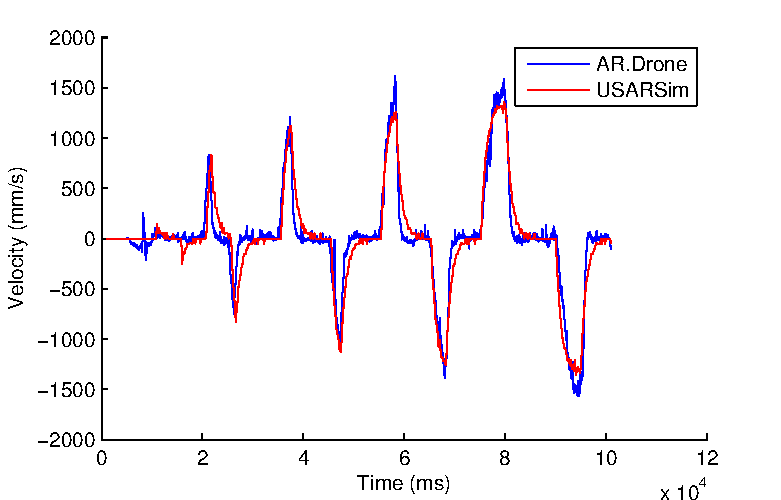
\includegraphics[width=11cm]{images/RYtdB-eps-converted-to.pdf}
\caption{Velocity of the real (blue) and simulated AR.Drone (red) on the same control pulses as shown in Figure~\ref{fig:RealResponse}.}

\label{fig:ComparisonOfResponse}
\end{figure}

As one can see, the acceleration has for the real and simulated AR.Drone nearly the same slope. The deceleration of the simulated AR.Drone is slightly lower. In the real AR.Drone the feedback loop (based on the optical flow of the ground camera) actively decelerates the system. Overall, the dynamic behavior of the simulator closely resembles the dynamic behavior of the real system. Additionally, tests with more complex maneuvers (horizontal and vertical square) have been recorded, but unfortunately not yet analyzed in detail.


	\section{Pose estimation}
	\section{Mapping}
An experiment has been carried out to evaluate the mapping approach.
This experiment is performed with the AR.Drone and the simulated AR.Drone using USARSim.

\begin{figure}[htb]
\centering
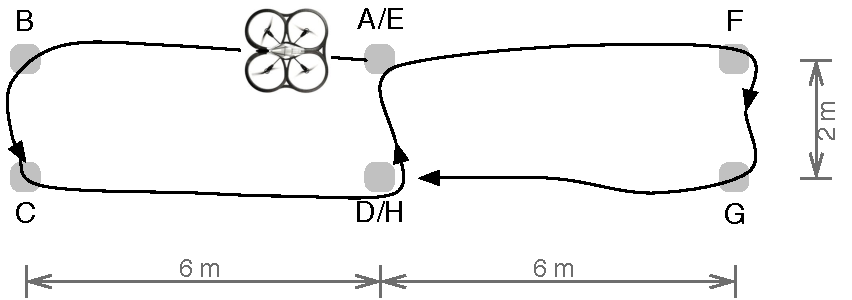
\includegraphics[width=13.0cm]{images/floorplan.pdf} %8cm te klein
\caption{Top view of the experiment's floorplan. The AR.Drone flew an 8-shape. The labels A-G represent six landmarks that provide ground truth to evaluate the accuracy of a map.}
\label{fig:exp_floorplan}
\end{figure}

A sports hall is used as indoor testing environment. This environment closely resembles the environment of the IMAV2011 indoor competitions.
Six magazines are laid out on the floor at the locations A, B, C, D, F, G in Figure \ref{fig:exp_floorplan}.
These magazines are used as landmarks that are easily recognizable in the map.
% Each landmark has a label (A, B, C, etc).
The distances between these landmarks are known, providing ground truth.
The AR.Drone flew in an 8-shape above the floor to capture an intermediate loop (point A and E in Figure \ref{fig:exp_floorplan}).
% also 8-shape to mimic the goal of the indoor competition.
In addition to the landmarks, the lines on the floor provide visual clues about the overall quality of a created map.
Care has been taken to mimic the gym floor in the simulated environment.
The floor of the simulated environment consists of an image taken at the IMAV2011 competitions. 
The image was taken from the gym tribune and warped with an image editor to remove the perspective view as much as possible.
Unfortunately, some warping artifacts are visible on the simulated gym floor.
%These artifacts are visible in the map that is created by the mapping method.

The mapping method is performed on the floor as described above. The distances between the landmarks inside the generated map (red lines) are compared to the know ground truth to compute the error of the map.

\begin{figure}[htb]
\centering
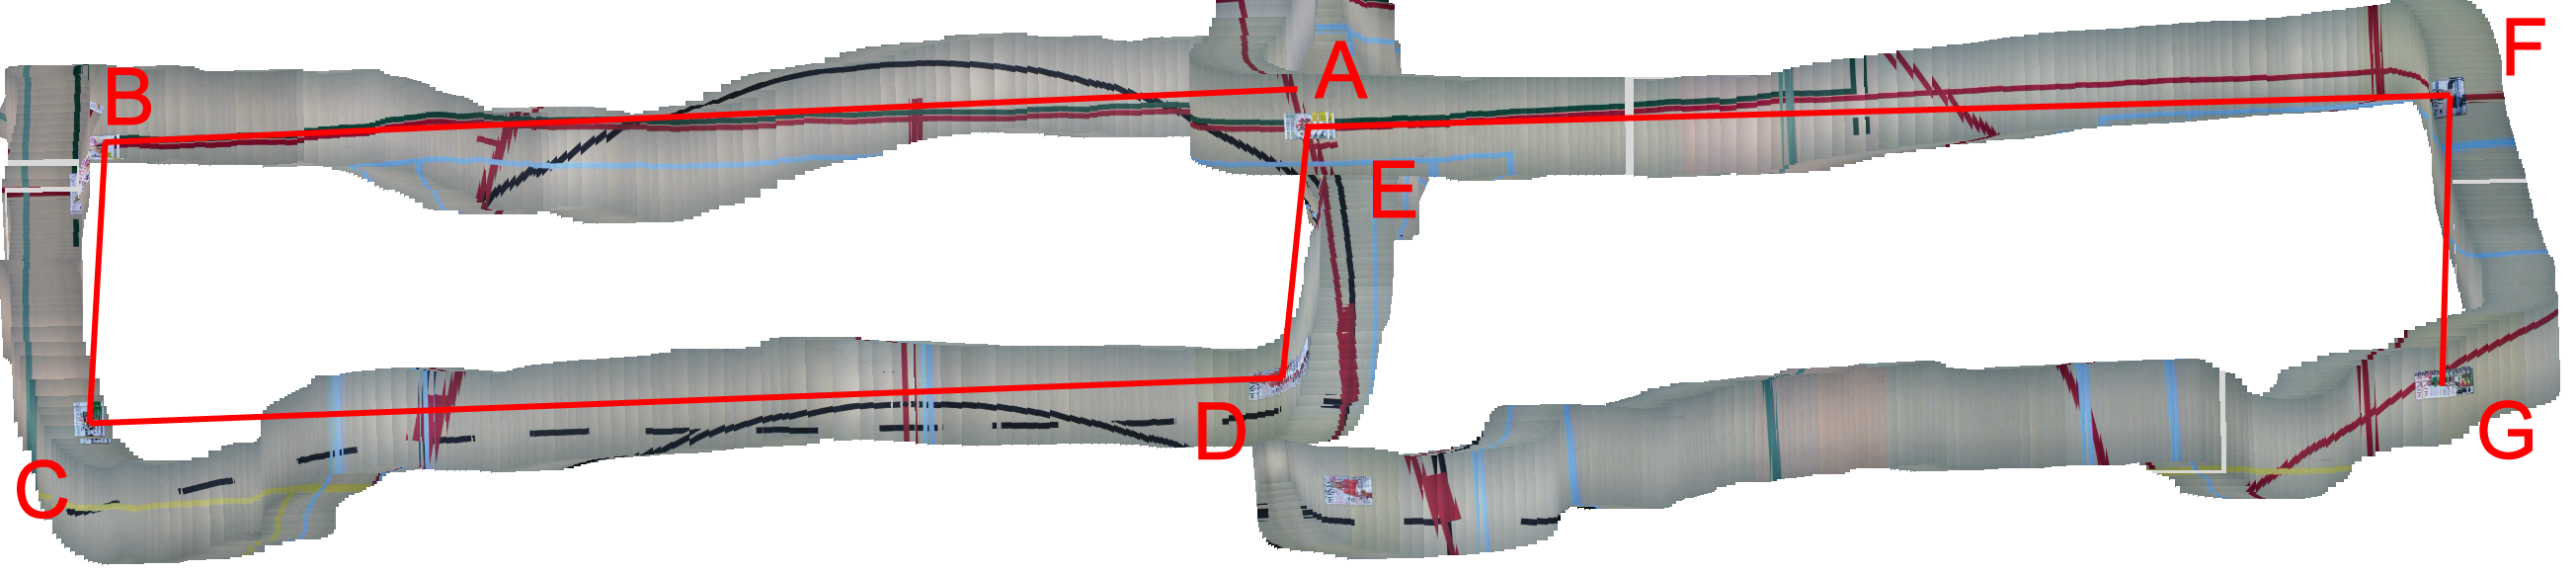
\includegraphics[width=\linewidth]{images/map_ardrone.png}
\caption{Visual map created by the mapping method. Camera images are taken by the AR.Drone, flying at approximately 70cm altitude.}
\label{fig:res_mapping_ardrone}
\end{figure}

\begin{figure}[htb]
\centering
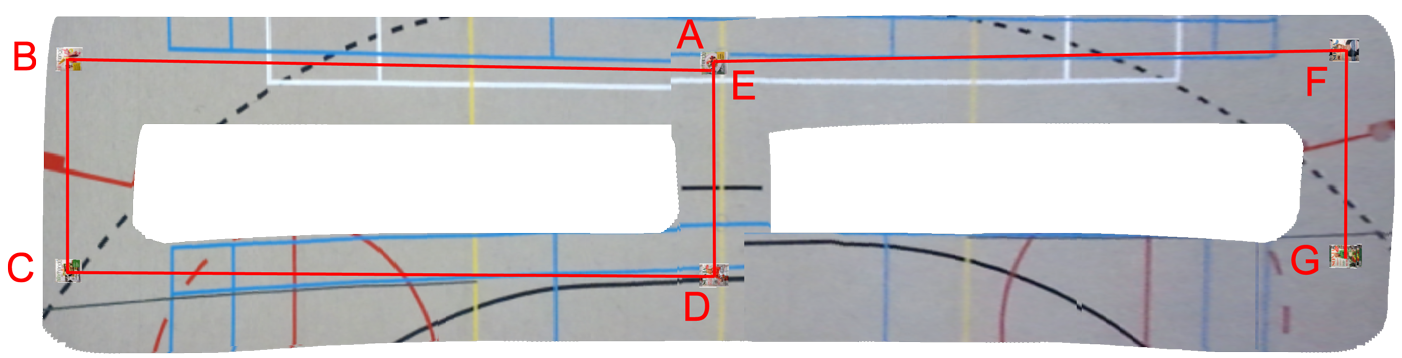
\includegraphics[width=14.8cm]{images/map_usarsim.png}
\caption{Visual map created by the mapping method. Camera images are taken by the simulated AR.Drone, flying at approximately 85cm altitude.}
\label{fig:res_mapping_usarsim}
\end{figure}


\begin{table}[htb!]
    \centering
    \begin{tabular}
        { | l | l | l | l | l | l | l | l | l |} 
	\hline
	landmarks & A-B & B-C & C-D & D-E & E-F & F-G & B-G & C-F \\
        \hline
        \textbf{AR.Drone} & & & & & & & & \\
	%\hline
	mean error (m) & 0.042 & 0.653 & 0.087 & 0.726 & 0.350 & 0.579 & 0.491 & 0.388  \\
	error (\%) & 0.71 & 32.65 & 1.44 & 36.28 & 5.84 & 28.95 & 4.03 & 3.19\\
	\hline
	\textbf{USARSim simulator} & & & & & & & & \\
	%\hline
	mean error (m) & 0.280 & 0.095 & 0.319 & 0.010 & 0.172 & 0.021 & 4.566 & 0.496 \\
	error (\%) & 4.66 & 4.74 & 5.31 & 4.98 & 2.85 & 1.1 & 3.75 & 4.1 \\
	\hline
    \end{tabular}
    \caption{Accuracy of the visual map by measuring the distance between landmarks. The maps are created using the AR.Drone (Figure \ref{fig:res_mapping_ardrone}) and the USARSim simulator (Figure \ref{fig:res_mapping_usarsim}) .}
    \label{tab:res_mapping}
\end{table}

%This experiment illustrates that the current mapping approach is able to produce a map in a controlled environment. 

The results of this experiment can be found in Table \ref{tab:res_mapping} and Figures \ref{fig:res_mapping_ardrone} (real AR.Drone) and \ref{fig:res_mapping_usarsim} (simulated AR.Drone).
Both the simulated and real AR.Drone produce a map with enough quality for
%human navigation
navigation in the IMAV Pylon challenge.
The visual map could be further optimized by a method equivalent to TORO \cite{Grisetti2007iros}.
The visual map created by the simulated AR.Drone contains fewer errors than the map of the real AR.Drone.
Despite the simulator's inertia measurements are noise-free, there are small errors in the map.
These errors are due to integrating the acceleration measurements to velocities and positions.
The largest errors are in the long stretches of the trajectory, because these parts of the trajectory are longer affected by integration errors due to the larger traveling times.

The position of the real AR.Drone was estimated using the AR.Drone's velocity estimates produced by the proprietary onboard filter.
This estimate is based on inertia measurements and optical flow obtained from the relative motion between camera frames.
These measurements suffer from noise, resulting in larger map errors.
The AR.Drone's proprietary optical flow algorithm is probably having difficulties with the gym floor.
When flying along a single line or parallel lines (e.g. path B-C in Figure \ref{fig:res_mapping_ardrone}), no apparent motion can be observed from the camera frames.
These circumstances mainly occured when flying along the short stretches in the trajectory, producing the largest errors in this direction.
This behavior is not observed for the simulated AR.Drone, because it lacks an optical flow method to estimate the velocity.


\begin{comment}
\textbf{How to integrate the white balancing paragraph? To explain visual differences between both maps?} \
Care has been taken to reproduce the circumstances in simulation as good as possible; the camera images in simulation are post-processed (decreased saturation, increased brightness, down-sampled resolution) to mimic the real images as close as possible. The difference between real and simulated visual map could also be explained by smoother movements between the frames in simulation. Yet, also here care has been taken to mimic the dynamics of the AR.Drone as close as possible (as described in Section \ref{sec:validation_results}). Visual inspection of the video stream shows that there are equivalent changes in the movements between frames. Our hypothesis is that the remaining difference between simulation and reality are due to the effect of automatic white balancing of the real camera. In the next experiment this hypothesis will be further studied.
\end{comment}


	\section{Localization}
Another experiment has been carried out to evaluate the localization approach.
This experiment resembles quite closely the IMAV Pylon Challenge. This experiment is performed with the simulated AR.Drone only to demonstrate the possibilities for localization when a reasonable accurate visual map (errors in the order of 5\%, as found in the previous section) is available. 
The USARSim simulator provides accurate ground truth that is used to evaluate the performance.

For this experiment, the trajectory from the mapping experiment (Figure \ref{fig:exp_floorplan}) is repeated several times.
%The map created in the previous experiment (Section \ref{sec:res_mapping}) is now used for localization.
Eleven 8-shapes (called rounds) were flown autonomously.
During the first round, the map is created.
The remaining 10 rounds are flown with mapping turned off and localization turned on.
The $x, y$ and $z$ distance between the estimated location and real location (ground truth) is measured and used as error measure.
This experiment is repeated with localization turned off, meaning that the location is estimated using the inertia measurements only.

\begin{figure}[htb!]
\centering
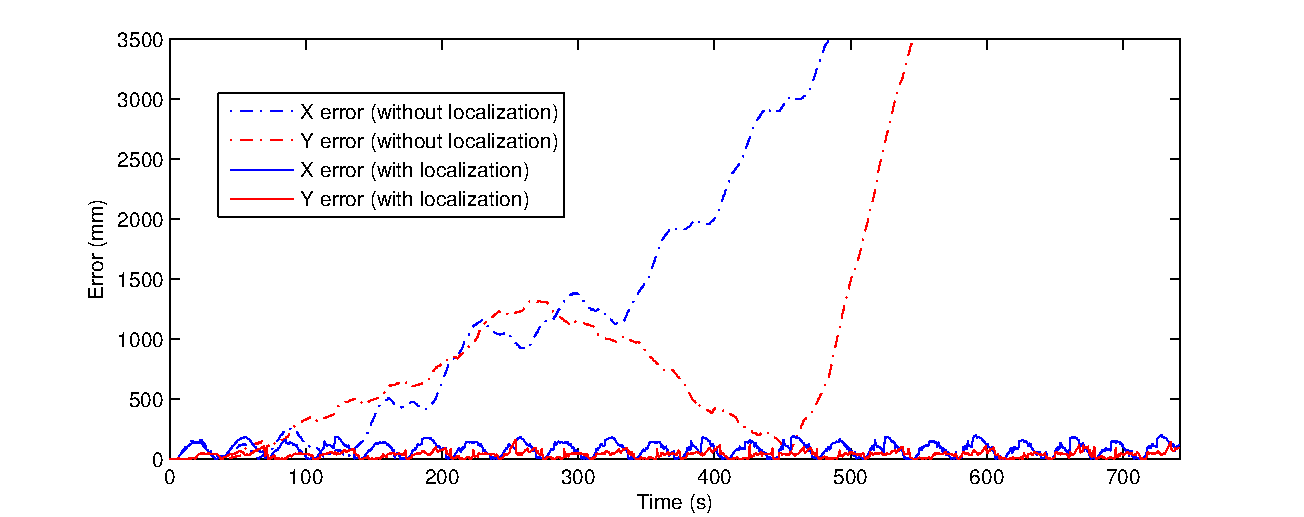
\includegraphics[width=14cm]{images/error_loc-eps-converted-to.pdf}
\caption{Error between the estimated position and actual position (ground truth). The experiment is performed  with visual localization (solid lines) and repeated without visual localization (dashed lines).}
\label{fig:res_localization_error}
\end{figure}

\begin{figure}[htb!]
\centering
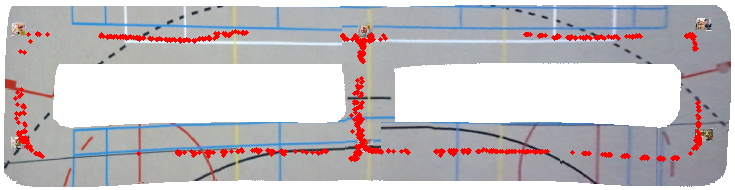
\includegraphics[width=14.0cm]{images/ardrone_map_loc_positions.png}
\caption{Visual map with localization positions. Each red dot represents a position of the AR.Drone where visual localization was performed.}
\label{fig:res_loc_positions}
\end{figure}

The results of this experiment can be found in Figure \ref{fig:res_localization_error}.
Without localization, the error of the estimated position increases over time (dashed lines).
Around 280 seconds the drift in Y direction seems to reverse.
This drift in reversed direction is causing a decreasing Y error until the error is completely compensated.
However, the drift is continuing and the error increases again.
With localization turned on, the error remains low during the whole flight.
The first 75 seconds correspond to the first 8-shape that is used create a map.
During this mapping flight, the error of the estimated position increases and the quality (accuracy) of the map decreases.
Again, reversed drifting causes a temporary drop in error around 35 seconds.
The repetitive error pattern suggests that the error of the estimated position largely depends on the quality (accuracy) of the map, if localization can be performed regularly.

Figure \ref{fig:res_loc_positions} indicates the positions where the AR.Drone was able to localize itself.
Localization was performed at almost every position of the 8-shape trajectory.
Not only the magazines, but also the lines on the gym floor provide sufficient information for localization.
At some positions localization was not possible, because the camera observed insufficient image features.
For example, when lines without intersections are observed.
%\textit{From these results we [conclude] that our localization method can be deployed for the IMAV indoor competitions.}
These results confirm that the localization method is able to deal with circumstances encountered during the IMAV competition.


	\section{Elevation mapping}